\documentclass{beamer}

\setbeamercolor{framesubtitle}{fg=black}
\setbeamercolor{frametitle}{fg=white}
\setbeamercolor{navigation symbols}{fg=white, bg=white}
\setbeamercolor{section in toc}{fg=black}
\setbeamercolor{title}{fg=black}
\setbeamerfont{framesubtitle}{series=\bfseries, size=\large}
\setbeamerfont{frametitle}{series=\bfseries}
\setbeamerfont{institute}{size=\normalsize}
\setbeamerfont{section in toc}{series=\bfseries}
\setbeamerfont{subsection in toc}{series=\bfseries}
\setbeamerfont{title}{series=\bfseries}
\setbeamertemplate{frametitle}[default][right]
\setbeamertemplate{section in toc shaded}[default][50]
\setbeamertemplate{section in toc}[sections numbered]
\setbeamertemplate{sidebar right}{}
\setbeamertemplate{subsection in toc shaded}[default][50]
\setbeamertemplate{subsection in toc}[subsections numbered]

\addtobeamertemplate{footline}{%
	\hfill\usebeamertemplate***{navigation symbols}
	\hspace*{1em}\par\vspace{1pt}
}{}

\usepackage[UTF8]{ctex}
\usepackage[sort&compress]{natbib}
\usepackage{graphicx}
\usepackage{verbatim}
\usepackage{listings}


\AtBeginSection[]
{%
	\begin{frame}<beamer>
	\frametitle{目录}
	\tableofcontents[currentsection]
\end{frame}
}



\title{Aomi Online 性能测试報告}
\author{author:xiaoyulong }
\institute{Aomi}
\date{\today}

\begin{document}

\usebackgroundtemplate{%
	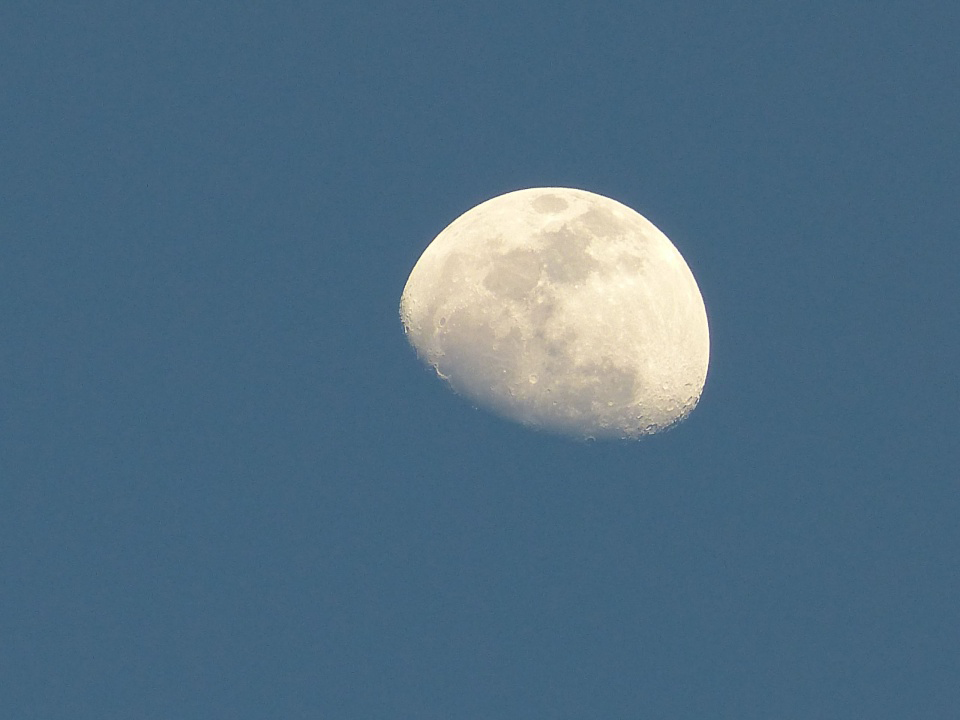
\includegraphics[width=\paperwidth,height=\paperheight]{img/title.png}
}

\frame{\titlepage}

\usebackgroundtemplate{%
	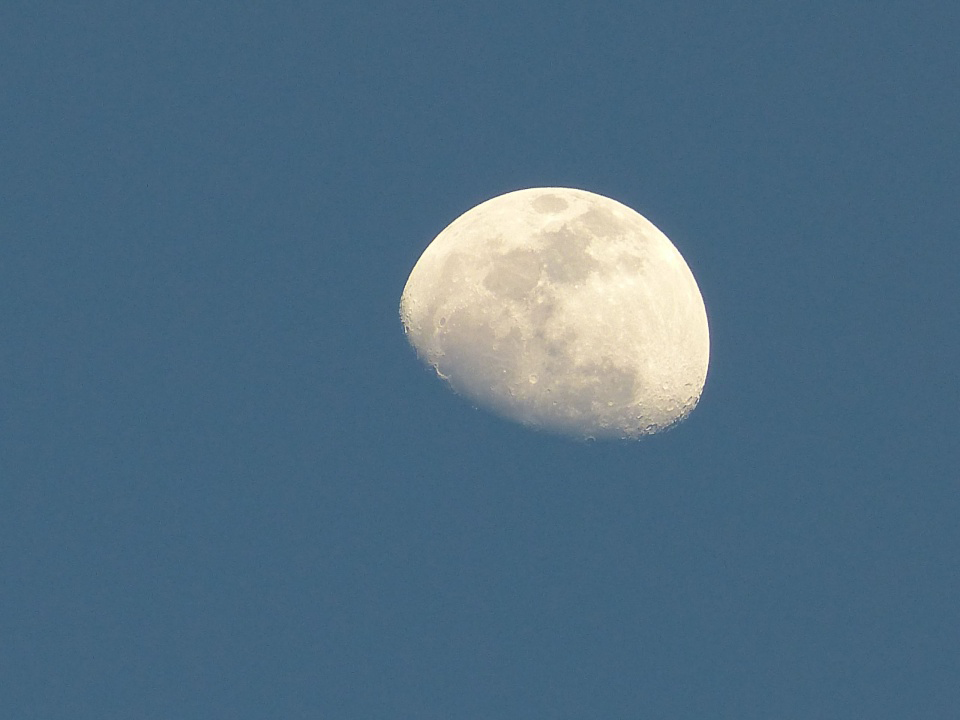
\includegraphics[width=\paperwidth,height=\paperheight]{img/content.png}
}

\begin{comment}
1.写测试背景

2.测试目标

3.测试范围

4.测试环境

5.测试数据

6.测试标准(重点)

7.测试进度

8.测试结果

9.测试结论*

\end{comment} 

\section{第一章节 测试背景}




\begin{frame}
\frametitle{测试背景}
\begin{itemize}
	\item 参数配置
	\small
	
	      Aomi自创立以来,除了对功能要求很高以外,对性能要求也越来越高。
      Aomi性能测试在不断向前发展,横向、纵向都在不断深入、拓宽,不断提出更高要求。
      
      
      一个应用
      的性能由多方面因素决定,这样就加大了对性能测试和性能调优的难度,也扩大了性能测试
      的广度,这是一个挑战。专业的测试需要专业的格式,	  
	    	
\end{itemize}
\end{frame}



\section{第二章节 测试目标}



\begin{frame}
\frametitle{Aomi 基准性能}
\begin{itemize}
	\item 基准性能
	\small
	  更有效利用環境,提高POC
	
	
	
	  
	
\end{itemize}
\end{frame}

\begin{frame}
\frametitle{Aomi 性能}
\begin{itemize}
	\item 基准性能
	\small
	
	日常性能支持,業務支撐
	
	
	
	
	
\end{itemize}
\end{frame}





\begin{frame}
\frametitle{Aomi 秒殺 推送}
\begin{itemize}
	\item 基准性能
	\small
	
	
	支持秒殺活動,支持推送
	
	
	
	
\end{itemize}
\end{frame}

\begin{frame}
\frametitle{Aomi 極限}
\begin{itemize}
	\item 基准性能
	\small
	
	
	配置網關限流,避免負載導致系統宕機
	
	
	
	
\end{itemize}
\end{frame}



\section{第三章节 测试范围}



\begin{frame}
\frametitle{Aomi 當前的架構和數據隔離問題,暫時}
\begin{itemize}
	\item 基准性能
	\small
	
	
	Aomi 當前的架構和數據隔離問題,暫時只支持查詢接口的性能測試。
	
	
	
	
\end{itemize}
\end{frame}






\section{第四章节 测试环境 测试数据}

\begin{frame}
\frametitle{测试环境 基本架構}
\begin{figure}[ht]
	
	\centering
	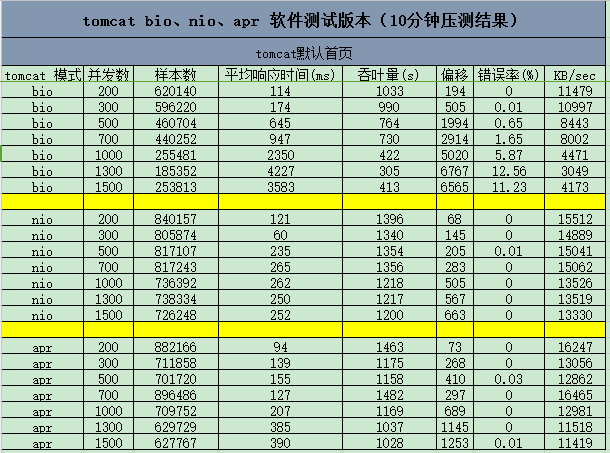
\includegraphics[scale=0.45]{img/benchmark.png}
	\caption{基准性能图表}
	\label{fig:pathdemo1}
\end{figure}

\end{frame}


\begin{frame}
\frametitle{Aomi 當前的架構和數據隔離問題,暫時}
\begin{itemize}
	\item 基准性能
	\small
	
	
	Aomi 當前的架構和數據隔離問題,暫時只支持查詢接口的性能測試。
	
	
	
	
\end{itemize}
\end{frame}



\section{参考文献}

\begin{frame}[allowframebreaks]
\frametitle{参考文献}
\small
\bibliographystyle{plain}
\bibliography{slide}
https://blog.csdn.net/mrleeapple/article/details/80420395

https://zh.wikipedia.org/wiki/Apache%E5%8F%AF%E7%A7%BB%E6%A4%8D%E8%BF%90%E8%A1%8C%E6%97%B6
\end{frame}

\begin{frame}[allowframebreaks]
\frametitle{参考文献}
\centering
\begin{tabular}{|l|c|r|}
\hline 
\large	JDK版本 &  \large 默认GC&  \large 性能 \\
\hline 
JDK8 & G1非并发 &  GC \\
\hline 
JDK11 & G1并发 & GC \\
\hline 
openjdk8 & G1非并发& GC  \\
\hline 
openjdk11& G1并发 & GC \\
\hline
\end{tabular}
\end{frame}

\begin{frame}[allowframebreaks]
\frametitle{JDK版本 与GC}
\centering
\begin{tabular}{|l|c|r|}
\hline 
\large	Connector&  \large 版本要求&  \large IO \\
\hline 
Http11Protocol & 7、8、9 & BIO \\
\hline 
Http11NioProtocol & 7、8、9 & NIO \\
\hline 
Http11Nio2Protocol & 8、9& NIO2  \\
\hline 
Http11AprProtocol& 7、8、9 & APR \\
\hline
\end{tabular}
\end{frame}



\section{第五章节 测试标准(重点)}






\section{参考文献}

\begin{frame}[allowframebreaks]
\frametitle{参考文献}
\small
\bibliographystyle{plain}
\bibliography{slide}
https://blog.csdn.net/mrleeapple/article/details/80420395

https://zh.wikipedia.org/wiki/Apache%E5%8F%AF%E7%A7%BB%E6%A4%8D%E8%BF%90%E8%A1%8C%E6%97%B6
\end{frame}

\begin{frame}[allowframebreaks]
\frametitle{参考文献}
\centering
\begin{tabular}{|l|c|r|}
\hline 
\large	JDK版本 &  \large 默认GC&  \large 性能 \\
\hline 
JDK8 & G1非并发 &  GC \\
\hline 
JDK11 & G1并发 & GC \\
\hline 
openjdk8 & G1非并发& GC  \\
\hline 
openjdk11& G1并发 & GC \\
\hline
\end{tabular}
\end{frame}

\begin{frame}[allowframebreaks]
\frametitle{JDK版本 与GC}
\centering
\begin{tabular}{|l|c|r|}
\hline 
\large	Connector&  \large 版本要求&  \large IO \\
\hline 
Http11Protocol & 7、8、9 & BIO \\
\hline 
Http11NioProtocol & 7、8、9 & NIO \\
\hline 
Http11Nio2Protocol & 8、9& NIO2  \\
\hline 
Http11AprProtocol& 7、8、9 & APR \\
\hline
\end{tabular}
\end{frame}




\section{第六章节 测试结果}



\begin{frame}
\frametitle{Tomcat 基准性能}
\begin{figure}[ht]

\centering
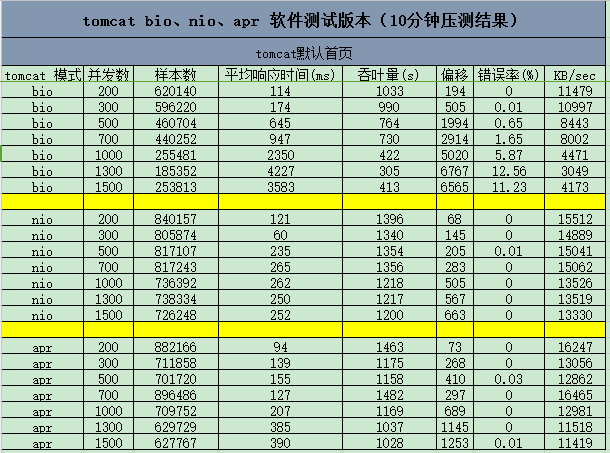
\includegraphics[scale=0.45]{img/benchmark.png}
\caption{基准性能图表}
\label{fig:pathdemo1}
\end{figure}

\end{frame}


\section{参考文献}

\begin{frame}[allowframebreaks]
\frametitle{参考文献}
\small
\bibliographystyle{plain}
\bibliography{slide}
https://blog.csdn.net/mrleeapple/article/details/80420395

https://zh.wikipedia.org/wiki/Apache%E5%8F%AF%E7%A7%BB%E6%A4%8D%E8%BF%90%E8%A1%8C%E6%97%B6
\end{frame}

\begin{frame}[allowframebreaks]
\frametitle{参考文献}
\centering
\begin{tabular}{|l|c|r|}
\hline 
\large	JDK版本 &  \large 默认GC&  \large 性能 \\
\hline 
JDK8 & G1非并发 &  GC \\
\hline 
JDK11 & G1并发 & GC \\
\hline 
openjdk8 & G1非并发& GC  \\
\hline 
openjdk11& G1并发 & GC \\
\hline
\end{tabular}
\end{frame}

\begin{frame}[allowframebreaks]
\frametitle{JDK版本 与GC}
\centering
\begin{tabular}{|l|c|r|}
\hline 
\large	Connector&  \large 版本要求&  \large IO \\
\hline 
Http11Protocol & 7、8、9 & BIO \\
\hline 
Http11NioProtocol & 7、8、9 & NIO \\
\hline 
Http11Nio2Protocol & 8、9& NIO2  \\
\hline 
Http11AprProtocol& 7、8、9 & APR \\
\hline
\end{tabular}
\end{frame}




\section{第七章节 测试结论 分析}



\begin{frame}
\frametitle{Tomcat 基准性能}
\begin{figure}[ht]

\centering
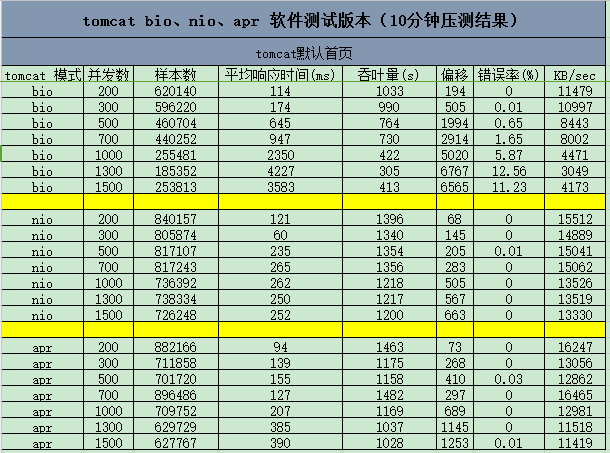
\includegraphics[scale=0.45]{img/benchmark.png}
\caption{基准性能图表}
\label{fig:pathdemo1}
\end{figure}

\end{frame}


\section{参考文献}

\begin{frame}[allowframebreaks]
\frametitle{参考文献}
\small
\bibliographystyle{plain}
\bibliography{slide}
https://blog.csdn.net/mrleeapple/article/details/80420395

https://zh.wikipedia.org/wiki/Apache%E5%8F%AF%E7%A7%BB%E6%A4%8D%E8%BF%90%E8%A1%8C%E6%97%B6
\end{frame}

\begin{frame}[allowframebreaks]
\frametitle{参考文献}
\centering
\begin{tabular}{|l|c|r|}
\hline 
\large	JDK版本 &  \large 默认GC&  \large 性能 \\
\hline 
JDK8 & G1非并发 &  GC \\
\hline 
JDK11 & G1并发 & GC \\
\hline 
openjdk8 & G1非并发& GC  \\
\hline 
openjdk11& G1并发 & GC \\
\hline
\end{tabular}
\end{frame}

\begin{frame}[allowframebreaks]
\frametitle{JDK版本 与GC}
\centering
\begin{tabular}{|l|c|r|}
\hline 
\large	Connector&  \large 版本要求&  \large IO \\
\hline 
Http11Protocol & 7、8、9 & BIO \\
\hline 
Http11NioProtocol & 7、8、9 & NIO \\
\hline 
Http11Nio2Protocol & 8、9& NIO2  \\
\hline 
Http11AprProtocol& 7、8、9 & APR \\
\hline
\end{tabular}
\end{frame}

\section*{}


\usebackgroundtemplate{%
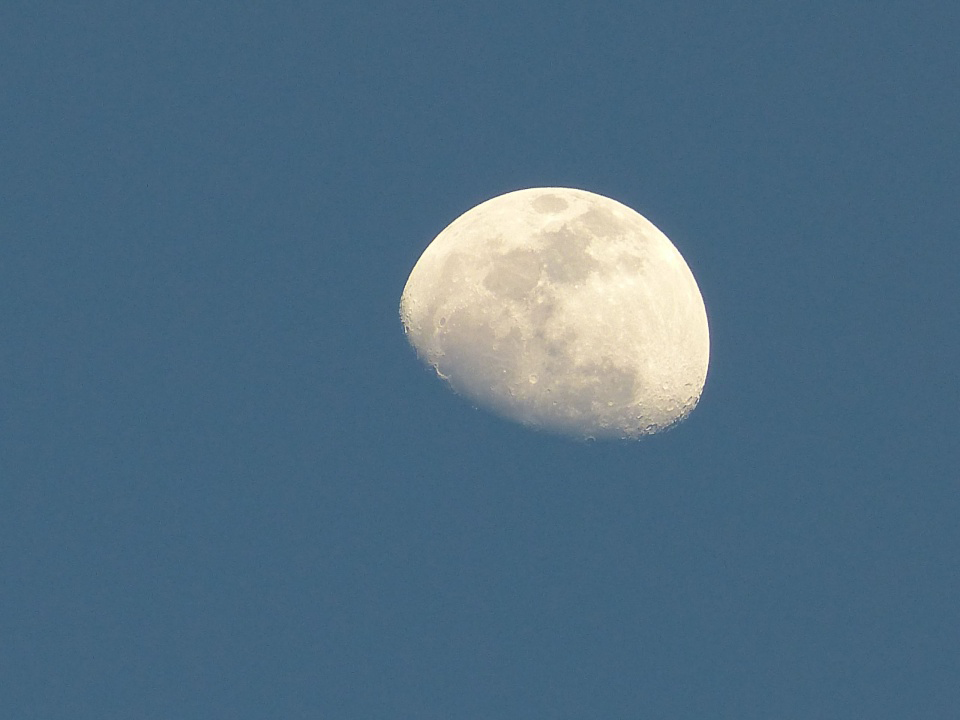
\includegraphics[width=\paperwidth,height=\paperheight]{img/title.png}
}


\begin{frame}
\centering
\Huge Q \& A
\end{frame}

\begin{frame}
\centering
\Huge Thank you !
\end{frame}

\end{document}
